\documentclass{beamer}
\usetheme{Boadilla}
\usecolortheme{sidebartab}
\beamertemplatenavigationsymbolsempty
\setbeamertemplate{footline}[frame number]
\usepackage{hyperref} 
\usepackage{graphicx}
\usepackage{color}
\usepackage{booktabs}
\usepackage{listings}
\usepackage{soul}
\usepackage{tikz}
\usepackage[utf8]{inputenc}
\usepackage{CJKutf8}
\usetikzlibrary{shapes.geometric}

\definecolor{gray}{rgb}{0.4,0.4,0.4}
\definecolor{darkblue}{rgb}{0.0,0.0,0.6}
\definecolor{cyan}{rgb}{0.0,0.6,0.6}

\lstset{
	basicstyle=\ttfamily,
	columns=fullflexible,
	showstringspaces=false,
	commentstyle=\color{gray}\upshape
}

\tikzset{node style/.style={
		draw=blue,
		thick,
		fill=blue!70,
		text=white,
		ellipse,
		minimum width=2cm,
		minimum height=0.75cm,
		font=\small,
		outer sep=3pt,
	},
	blank style/.style={
		draw=black,
		thick,
		fill=white,
		text=white,
		ellipse,
		minimum width=2cm,
		minimum height=0.75cm,
		font=\small,
		outer sep=3pt,
	},
	literal style/.style={
		draw=red,
		thick,
		fill=red!70,
		text=white,
		rectangle,
		minimum width=2cm,
		minimum height=0.75cm,
		font=\small,
		outer sep=3pt,
	},
	edge style/.style={
		#1,
		text=black,
		font=\footnotesize,
		above
	}
}

\makeatletter
\newcommand\SoulColor{%
	\let\set@color\beamerorig@set@color
	\let\reset@color\beamerorig@reset@color}
\makeatother

\lstset{language=XML}

\title{RDF: Fortgeschrittene Themen}
\author{Markus Stocker}
\date{7. Mai 2018}

\begin{document}

\maketitle

\begin{frame}{Rekapitulation}
	
	\begin{itemize}
		\item Was ist ein RDF Tripel?
		\item Wozu benötigt man eine Serialisierung?
		\item Welche RDF Syntax liest sich am besten?
		\item Welche Gründe sprechen für RDF/XML?
	\end{itemize}
	
\end{frame}

\begin{frame}{Übersicht}
	
	\begin{itemize}
		\item Das Prädikat \texttt{rdf:type}
		\item Datentypen
		\item Angabe zu natürlicher Sprache (\emph{language tag})
		\item Listen in RDF
		\item Reifizierung (\emph{reification})
	\end{itemize}
	
\end{frame}

\begin{frame}[fragile]{Das Prädikat \texttt{rdf:type}}
	
	\begin{itemize}
		\item Das \texttt{rdf:type} Prädikat ist Teil des RDF Vokabular
		\item Es wird benutzt um einem URI einen Typ zuzuordnen
		\item Die URI referenzierte Ressource gehört dem entsprechenden Typ
		\item In Turtle auch mit `\texttt{a}' kürzbar
		\item Solche Typisierung im Semantischen Web von zentraler Bedeutung
		\item Mehr dazu in RDF Schema
	\end{itemize}
	
	\small
	\begin{lstlisting}
  @prefix ex: <http://example.org#> .
  @prefix rdf: <http://www.w3.org/1999/02/22-rdf-syntax-ns#> .
    
  ex:Earth rdf:type ex:Planet .
  
  ex:Mars a ex:Planet . 
	\end{lstlisting}
	
\end{frame}

\begin{frame}{Datentypen}
	
	\begin{itemize}
		\item Literale werden grundsätzlich als Zeichenfolge interpretiert
		\item Dies ist in praktischen Anwendungen unzureichend
		\item Man benötig weit mehr an Datentypen, z.B. Nummern oder Zeiten
		\item Datentyp hat Auswirkungen auf die Interpretation eines Wertes
		\item Klassisches Beispiel: ``02'', ``2'', ``20``
		\item Sortierung als Nummern oder Zeichenfolgen ist unterschiedlich
	\end{itemize}
	
\end{frame}

\begin{frame}{Datentypen}
	
	\begin{itemize}
		\item RDF Literale können Datentyp explizit angeben
		\item Solche Literale werden \emph{typisierte} Literale genannt
		\item Datentypen sind mittels URI identifiziert
		\item Beispiele aus XML Schema
		\begin{itemize}
			\item \texttt{http://www.w3.org/2001/XMLSchema\#string}
			\item \texttt{http://www.w3.org/2001/XMLSchema\#date}
			\item \texttt{xsd:int}
		\end{itemize}
		\item XML Schema Datetypen sind weit verbreitet (für elementare Typen)
		\item Datentypen können allerdings beliebig erweitert werden
		\item Beispiel: \texttt{http://www.opengis.net/ont/geosparql\#wktLiteral}
		\item Bedeutet nicht, dass diese von einer Software auch unterstützt werden
		\item Selbst XML Schema Datentypen nicht zwingend unterstützt
	\end{itemize}
	
\end{frame}

\begin{frame}{Datentypen}
	
	\begin{itemize}
		\item Syntaktisch ungleiche Literale können semantisch gleich sein
		\item Datentypen ermöglichen solch differenzierte Handhabung
		\item Beispiel
		\begin{itemize}
			\item Die Literale \texttt{3.14}, \texttt{+03.14}, \texttt{3.140} sind syntaktisch ungleich
			\item Als untypisierte Literale werden diese ungleich behandelt
			\item Als typisierte Literale (\texttt{xsd:decimal}) sind sie semantich gleich
			\item Somit ist \texttt{decimal("3.14") == decimal("3.140")} wahr
		\end{itemize}
	\end{itemize}
	
\end{frame}

\begin{frame}[fragile]{Datentypen}
	
	\begin{itemize}
		\item Typisierte Literale müssen entsprechend Serialisiert werden
		\item In graphischer Darstellung wird meist \texttt{"..."\^{}\^{}<...>} verwendet
		\item Notation auch von Turtle und N-Triples Syntaxen verwendet
	\end{itemize}
	
	\vspace{1cm}
	
	\centering
	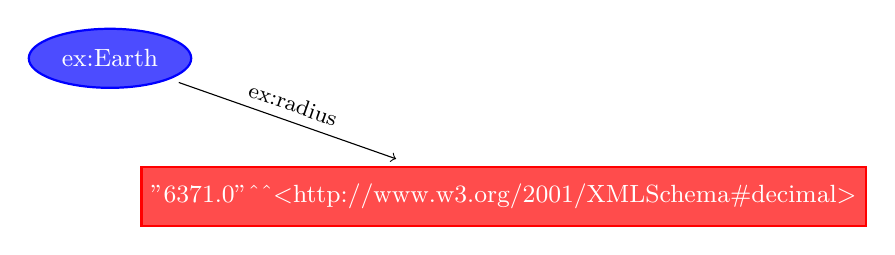
\begin{tikzpicture}[node distance=5cm]
	\node[node style] (Earth) {ex:Earth};
	\node[literal style, right of=Earth,yshift=-5em] (Radius) {"6371.0"\^{}\^{}$<$http://www.w3.org/2001/XMLSchema\#decimal$>$} 
	edge [<-] node[edge style=sloped,above]{ex:radius} (Earth);;
	\end{tikzpicture}
	
\end{frame}

\begin{frame}[fragile]{Datentypen: Turtle und N-Triples}
	
	\small
	\begin{lstlisting}
  @prefix ex: <http://example.org#> .
  @prefix xsd: <http://www.w3.org/2001/XMLSchema#> . 
		
  ex:Earth ex:radius "6371.0"^^xsd:decimal ;
    ex:label "Earth"^^<http://www.w3.org/2001/XMLSchema#string> .
		\end{lstlisting}
		
	\vspace{0.2cm}
	
	\centering\noindent\rule{8cm}{0.4pt}
	
	\vspace{0.2cm}
	
	\small
	\begin{lstlisting}
  <http://example.org#Earth> 
    <http://example.org#radius> 
      "6371.0"^^<http://www.w3.org/2001/XMLSchema#decimal> .
	\end{lstlisting}
	
\end{frame}

\begin{frame}[fragile]{Datentypen: RDF/XML}
	
	\small
	\begin{lstlisting}
  <!DOCTYPE rdf:RDF[
    <!ENTITY xsd 'http://www.w3.org/2001/XMLSchema#'>
    <!ENTITY ex 'http://example.org#'>
  ]>
    
  <rdf:RDF xmlns:rdf="http://www.w3.org/1999/02/22-rdf-syntax-ns#"
            xmlns:ex="http://example.org#">
	
    <rdf:Description rdf:about="&ex;Earth">
      <ex:radius rdf:datatype="&xsd;decimal">6371.0</ex:radius>
    </rdf:Description>
	
  </rdf:RDF>		
	\end{lstlisting}
	
\end{frame}

\begin{frame}[fragile]{Der RDF Datentyp \emph{XMLLiteral}}
	
	\begin{itemize}
		\item \texttt{rdf:XMLLiteral} ist ein in RDF eingebauter Datentyp
		\item Einbindung von XML als Werte in RDF Literale
	\end{itemize}
	
	\small
	\begin{lstlisting}		
  <rdf:RDF xmlns:rdf="http://www.w3.org/1999/02/22-rdf-syntax-ns#"
            xmlns:ex="http://example.org#">
		
    <rdf:Description rdf:about="http://example.org#Earth">
      <ex:radius rdf:parseType="Literal">
        <length unit="km">6371.0</length>
      </ex:radius>
    </rdf:Description>
		
  </rdf:RDF>		
	\end{lstlisting}
	
\end{frame}

\begin{frame}{Angabe zu Natürlicher Sprache (\emph{language tag})}
	
	\begin{itemize}
		\item Untypisierte Literale können eine Sprachangabe haben
		\item Wie der Datentyp ist auch dieser \emph{tag} Teil des Literals
		\item Sprich es wird kein weiteres Tripel dafür benötigt
		\item Die Sprachangabe ist für typisierte Literale nicht erlaubt
		\item Typisierte Literale gelten als Sprachunabhängig
	\end{itemize}
	
\end{frame}

\begin{frame}[fragile]{Angabe zu Natürlicher Sprache (\emph{language tag})}
	
	\small
	\begin{lstlisting}
  @prefix ex: <http://example.org#> .
	
  ex:Earth ex:label "Earth"@en, "Erde"@de, "Terra"@it .
	\end{lstlisting}
	
	\vspace{0.2cm}
	
	\centering\noindent\rule{8cm}{0.4pt}
	
	\vspace{0.2cm}
	
	\small
	\begin{lstlisting}	
  <rdf:RDF xmlns:rdf="http://www.w3.org/1999/02/22-rdf-syntax-ns#"
            xmlns:ex="http://example.org#">

    <rdf:Description rdf:about="http://example.org#Earth">
      <ex:label xml:lang="en">Earth</ex:label>
      <ex:label xml:lang="de">Erde</ex:label>
      <ex:label xml:lang="it">Terra</ex:label>
    </rdf:Description>

  </rdf:RDF>		
	\end{lstlisting}
	
\end{frame}

\begin{frame}[fragile]{Quiz: Wieviele Tripel?}
	
	\small
	\begin{lstlisting}
  @prefix ex: <http://example.org#> .
  @prefix xsd: <http://www.w3.org/2001/XMLSchema#> . 
	
  ex:Earth ex:label "Earth", "Earth"@en, "Earth"^^xsd:string .
	\end{lstlisting}
	
\end{frame}

\begin{frame}{Listen in RDF}
	
	\begin{itemize}
		\item Daten werden oft in listenartige Strukturen organisiert
		\item RDF stellt dafür verschiedene Konstrukte zur Verfügung
		\item Für offene (\emph{containers}) und geschlossene (\emph{collections}) Listen
		\item Es handelt sich hier nur um kürzungen für RDF Graphen
		\item Also \emph{``syntactic sugar''} für eine ansonsten (etwas) längere Form
	\end{itemize}
	
\end{frame}

\begin{frame}{Offene Listen: \emph{Containers}}
	
	\begin{itemize}
		\item Es gibt drei Arten von \emph{container}
		\begin{itemize}
			\item \emph{rdf:Seq}: Geordnete Liste
			\item \emph{rdf:Bag}: Ungeordnete Liste
			\item \emph{rdf:Alt}: Liste an alternativen
		\end{itemize}
		\item Diese Konstrukte haben nur informelle Semantik (Bedeutung)
 		\item Eine Anwendung kann die zusätzliche Information wahrnehmen
 		\item Die Anwendung muss das aber nicht
	\end{itemize}
	
\end{frame}

\begin{frame}[fragile]{Offene Listen: Beispiel, RDF/XML, Spezielle Syntax}
	
	\small
	\begin{lstlisting}	
  <rdf:Description rdf:about="http://example.org#SolarSystem">
    <ex:planets>
      <rdf:Seq>
        <rdf:li rdf:resource="http://example.org#Mercury"/>
        <rdf:li rdf:resource="http://example.org#Venus"/>
        <rdf:li rdf:resource="http://example.org#Earth"/>
        <rdf:li rdf:resource="http://example.org#Mars"/>
      </rdf:Seq>
    </ex:planets>
  </rdf:Description>
	\end{lstlisting}
	
\end{frame}

\begin{frame}[fragile]{Offene Listen: Beispiel, Visuell, Ungekürzte Form}
	
	\centering
	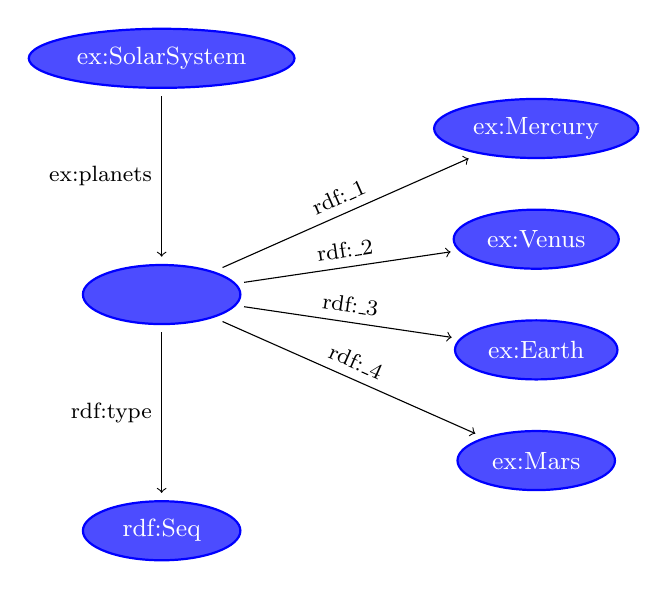
\begin{tikzpicture}[node distance=3cm]
	\node[node style] (SolarSystem) {ex:SolarSystem};
	
	\node[node style, below of=SolarSystem,xshift=0em] (Blank) {}
	edge [<-] node[edge style,left]{ex:planets} (SolarSystem);
	
	\node[node style, below of=Blank,xshift=0em] (Seq) {rdf:Seq}
	edge [<-] node[edge style,left]{rdf:type} (Blank);
	
	\node[node style, right of=Blank,yshift=6em,xshift=5em] (Mercury) {ex:Mercury}
	edge [<-] node[edge style=sloped,above]{rdf:\_1} (Blank);
	
	\node[node style, right of=Blank,yshift=2em,xshift=5em] (Venus) {ex:Venus}
	edge [<-] node[edge style=sloped,above]{rdf:\_2} (Blank);
	
	\node[node style, right of=Blank,yshift=-2em,xshift=5em] (Earth) {ex:Earth}
	edge [<-] node[edge style=sloped,above]{rdf:\_3} (Blank);
	
	\node[node style, right of=Blank,yshift=-6em,xshift=5em] (Mars) {ex:Mars}
	edge [<-] node[edge style=sloped,above]{rdf:\_4} (Blank);
	\end{tikzpicture}
	
\end{frame}

\begin{frame}[fragile]{Offene Listen: Beispiel, Turtle, Keine Spezielle Syntax}
	
	\small
	\begin{lstlisting}	
  @prefix ex: <http://example.org#> .
  @prefix rdf: <http://www.w3.org/1999/02/22-rdf-syntax-ns#> .
  
  ex:SolarSystem
    ex:planets [
      a rdf:Seq ;
      rdf:_1 ex:Mercury ;
      rdf:_2 ex:Venus ;
      rdf:_3 ex:Earth ;
      rdf:_4 ex:Mars 
    ] .
	\end{lstlisting}
	
\end{frame}

\begin{frame}{Geschlossene Listen: \emph{Collections}}
	
	\begin{itemize}
		\item Bei offenen Listen ist eine explizite Schliessung nicht möglich
		\item Man kann immer weitere Elemente hinzufügen (\texttt{rdf:\_n})
		\item Für geschlossene Listen stellt RDF \emph{collections} zur Verfügung
		\item Wie bei offenen Listen, handelt es sich auch hier um Kurzformen
		\item Sprich kurzgefasstere RDF Serialisierungen
	\end{itemize}
	
\end{frame}

\begin{frame}[fragile]{Geschlossene Listen: Beispiel, RDF/XML, Spezielle Syntax}
	
	\small
	\begin{lstlisting}	
  <rdf:Description rdf:about="http://example.org#SolarSystem">
    <ex:innerPlanets rdf:parseType="Collection">
      <rdf:Description rdf:about="http://example.org#Mercury"/>
      <rdf:Description rdf:about="http://example.org#Venus"/>
      <rdf:Description rdf:about=="http://example.org#Earth"/>
      <rdf:Description rdf:about=="http://example.org#Mars"/>
    </ex:innerPlanets>
  </rdf:Description>
	\end{lstlisting}
	
\end{frame}

\begin{frame}[fragile]{Geschlossene Listen: Beispiel, Visuell, Ungekürzte Form}
	
	\centering
	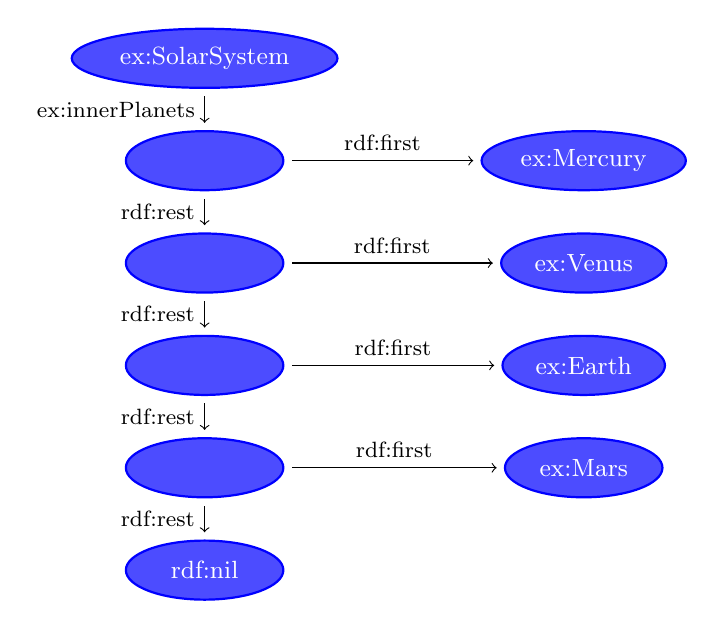
\begin{tikzpicture}[node distance=1.3cm]
	\node[node style] (SolarSystem) {ex:SolarSystem};
	
	\node[node style, below of=SolarSystem,xshift=0em] (Blank1) {}
	edge [<-] node[edge style,left]{ex:innerPlanets} (SolarSystem);
	
	\node[node style, right of=Blank1,xshift=10em] (Mercury) {ex:Mercury}
	edge [<-] node[edge style,above]{rdf:first} (Blank1);
	
	\node[node style, below of=Blank1,xshift=0em] (Blank2) {}
	edge [<-] node[edge style,left]{rdf:rest} (Blank1);
	
	\node[node style, right of=Blank2,xshift=10em] (Venus) {ex:Venus}
	edge [<-] node[edge style,above]{rdf:first} (Blank2);
	
	\node[node style, below of=Blank2,xshift=0em] (Blank3) {}
	edge [<-] node[edge style,left]{rdf:rest} (Blank2);
	
	\node[node style, right of=Blank3,xshift=10em] (Earth) {ex:Earth}
	edge [<-] node[edge style,above]{rdf:first} (Blank3);
	
	\node[node style, below of=Blank3,xshift=0em] (Blank4) {}
	edge [<-] node[edge style,left]{rdf:rest} (Blank3);
	
	\node[node style, right of=Blank4,xshift=10em] (Mars) {ex:Mars}
	edge [<-] node[edge style,above]{rdf:first} (Blank4);
	
	\node[node style, below of=Blank4,xshift=0em] (nil) {rdf:nil}
	edge [<-] node[edge style,left]{rdf:rest} (Blank4);
	\end{tikzpicture}
	
\end{frame}

\begin{frame}[fragile]{Geschlossene Listen: Beispiel, Turtle, Spezielle Syntax}
	
	\small
	\begin{lstlisting}	
  @prefix ex: <http://example.org#> .
  @prefix rdf: <http://www.w3.org/1999/02/22-rdf-syntax-ns#> .
	
  ex:SolarSystem
    ex:innerPlanets (
      ex:Mercury ex:Venus ex:Earth ex:Mars 
    ) .
	\end{lstlisting}
	
\end{frame}

\begin{frame}{Reifizierung (\emph{reification})}
	
	\begin{itemize}
		\item Aussagen über Aussagen
		\item Oder: Wenn die Aussage zum Gegenstand wird
		\item RDF: Wie sagt man etwas über ein Tripel aus?
		\item Dies wird mit Reifizierung ermöglicht
		\item Beispiel
		\begin{itemize}
			\item Eratosthenes schätzte den Erdradius auf 7018 km
			\item Teilaussage wie gehabt: \texttt{ex:Earth ex:radius "7018"}
			\item Aussage: \texttt{ex:Eratosthenes ex:estimated ?}
		\end{itemize}
	\end{itemize}
	
\end{frame}

\begin{frame}[fragile]{Reifizierung: Beispiel (Turtle)}
	
	\small
	\begin{lstlisting}	
  @prefix ex: <http://example.org#> .
  @prefix rdf: <http://www.w3.org/1999/02/22-rdf-syntax-ns#> .
		
  ex:Eratosthenes ex:estimated [
    rdf:type rdf:Statement ;
    rdf:subject ex:Earth ;
    rdf:predicate ex:radius ;
    rdf:object "7018"
  ] .
		\end{lstlisting}
	
\end{frame}

\begin{frame}[fragile]{Reifizierung: Beispiel (RDF/XML)}
	
	\small
	\begin{lstlisting}	
  <rdf:RDF xmlns:rdf="http://www.w3.org/1999/02/22-rdf-syntax-ns#"
            xmlns:ex="http://example.org#">

    <rdf:Description rdf:about="http://example.org#Eratosthenes">
      <ex:estimated>
        <rdf:Statement>
          <rdf:subject rdf:resource="http://example.org#Earth"/>
          <rdf:predicate rdf:resource="http://example.org#radius"/>
          <rdf:object>7018</rdf:object>
        </rdf:Statement>
      </ex:estimated>
    </rdf:Description>

  </rdf:RDF>
	\end{lstlisting}
	
\end{frame}

\begin{frame}{Reifizierung: Bemerkungen}
	
	\begin{itemize}
		\item Ein reifiziertes Tripel ist keine Aussage über dessen Gültigkeit
		\item Das Tripel selbst folgt aus der Reifizierung nicht
		\item Es folgt nicht, dass der Erdradius 7018 km ist
		\item Was Sinn macht, denn dies war die Schätzung von Eratosthenes
		\item Die in der Tat etwa um etwa 10\% falsch war
	\end{itemize}
	
\end{frame}

\begin{frame}{Zusammenfassung}
	
	\begin{itemize}
		\item Das wichtige Prädikat \texttt{rdf:type}
		\item Der Zweck wird im Kapitel RDF Schema nochmals deutlicher
		\item Wie auch schon für XML, sind Datentypen auch in RDF wichtig
		\item Das \emph{language tag} für untypisierte Literale
		\item Listen und Reifizierung in RDF
	\end{itemize}
	
\end{frame}

\end{document}